\documentclass[11pt,twoside,a4paper]{article}
\usepackage[hmargin=2cm, vmargin=2cm]{geometry}
\usepackage{microtype}
\usepackage{graphicx}
\usepackage{hyperref}
\usepackage[english]{babel}
\usepackage{setspace}
\usepackage{xcolor}
\usepackage{multicol}
\usepackage{float}
\usepackage{amsmath}
\usepackage{amssymb}
\usepackage[font=small,skip=2pt]{caption}
\usepackage[
backend=biber,
style=authoryear-comp,
]{biblatex}


\addbibresource{RMbibliography.bib}
\onehalfspacing
\parindent=0pt

\begin{document}
	\title{{\LARGE {\color{red}PLACEHOLDER-TITLE:} Functional Linear Regression in a Scalar-on-Function Setting with Applications to SOMETHING}}
	\author{Jonghun Baek, Jakob Juergens, Jonathan Willnow}
	\date{{\color{red}whenever}}
	\maketitle
	\vspace{1.5 cm}
	\begin{center}
		Research Module in Econometrics and Statistics \\
		Winter Semester 2021/2022
	\end{center}
	
	\newpage
	
	\tableofcontents
	
	\newpage
	
	\section{Colour Guide}
		\begin{itemize}
			\item {\color{red} RED}: is for general comments for your own text
			\item {\color{green} GREEN}: is for Jona's comments
			\item {\color{orange} ORANGE}: is for Jonghun's comments
			\item {\color{blue} BLUE}: is for Jakob's comments
		\end{itemize}
	
	\section{Introduction}
	
	\begin{itemize}
		\item Describe the idea of regressing a scalar on functional data
		\item Describing the difference to multiple linear regression intuitively
		\item Giving an intuitive example
	\end{itemize}	
	Functional Data Analysis (FDA) is a relatively new field {\color{red} (roots in the 1940s Grenander and Karhunen)} which is gaining more attention as researchers from different fields collect data that is functional in nature. Classical statistical methods can often process this data, but only FDA allows extracting information given by the smoothness of the underlying process (cf. \cite{levitin_introduction_2007}).
	 As \cite{kokoszka_introduction_2017} describe, FDA should be considered when one can view variables or units of a given data set as smooth curves or functions and the interest is in analyzing samples of curves (cf. \cite[S.~17]{kokoszka_introduction_2017}).\\
	 To motivate scalar-on-function regression, consider the case of a data set containing a scalar response and observations of an underlying continuous process. In economics, one application could be the regression of stock market correlations on the Global Crisis Index (GCI), where the regression allows to assess the relationship between the correlation and the GCI at every point within a window (cf. \cite{Das_2019}).\\
	 The focus of this paper is to introduce Functional Linear Regression (FLR) in a scalar-on-function setting. We will be using the standard FLR framework, which relates functional predictors to a scalar response as follows:
	 
	 \begin{equation}
	 	Y(\omega) = \alpha + \int_{0}^{1}{X(\omega)(s)\beta(s) \mathrm{d}s} + \epsilon(\omega),
	 	\qquad i = 1, ..., n
	 \end{equation}
 
	 where the $X_{i}$ are realizations of a random function $\mathbf{X}$, $Y_i$ are the corresponding realizations of the response variable and $\beta(s)$ is the coefficient function. The distinct feature of this framework is that the regressor is a function, which necessitates a different approach to estimation. As in the well-known framework of scalar linear regression, this is motivated by an interest in $\beta(s)$ for prediction. For instance, fluctuation in $X_i(s)$ at a point $s_0$ will not have any effect on $Y_i$ if $\beta(s_0)$ = 0. \\
	 Estimation of $\beta(s)$ is inherently an infinite-dimensional problem. In Section 2, after introducing the necessary theoretical concepts, we describe three methods of estimating a scalar coefficient function using a concept called truncated basis expansion. We report the results of the Monte-Carlo simulation regarding these three different methods in Section 3. Finally, in Section 4, we test the prediction of FLR in a real-world setting. {\color{red} (We may put some simple descriptions of results about each of MC and Application)}

	\section{Theory}
	In multivariate regression, data is often observed in the form of elements from Euclidean space, $\mathbb{R}^p$. However, the statistics derived from infinite-dimensional random functions cannot be defined on a finite dimensional space. To understand functional linear regression and the differences between the methods presented in this paper, it is therefore necessary to introduce some concepts and extend known aspects of linear regression theory to include functional objects. One integral concept in inferential statistics are random variables. Paraphrasing a definition by \cite{bauer_wahrscheinlichkeitstheorie_2020}, a random variable $X:\Omega \rightarrow \Omega'$ is an $\mathcal{A} \text{-} \mathcal{A'} \text{-measurable}$ function, where $(\Omega, \mathcal{A}, P)$ is a probability space and $(\Omega', \mathcal{A'})$ is a measure space.\\
	A typical case known to every undergraduate student of economics in less formal detail is $(\Omega', \mathcal{A'}) = (\mathbb{R}, \mathcal{B})$, where $\mathcal{B}$ is the canonical $\sigma$-algebra on the real numbers. As a first intuition, it is possible to imagine a similar concept where a random variable does not realize as an element of the real numbers but as a function in a function space. A formalization of this idea makes some more theoretical considerations necessary. The following theoretical introduction closely follows chapters 2.3 and 2.4 from \cite{hsing_theoretical_2015}. 
	
	\subsection{Inner Products and Hilbert Spaces}
	Let $\mathbb{V}$ be a vector space over some field of scalars $\mathbb{F}$. A function $\langle \cdot, \cdot \rangle : \mathbb{V} \times  \mathbb{V} \rightarrow \mathbb{F}$ is called an inner product, if $\forall v, v_1, v_2 \in \mathbb{V}$ and $a_1, a_2 \in \mathbb{F}$ the following properties hold.
	
	\begin{multicols}{2}
		\begin{enumerate}
			\item $\langle v, v \rangle \geq 0$
			\item $\langle v, v \rangle = 0$ if $v = 0$
			\item $\langle a_1 v_1 + a_2 v_2, v \rangle = a_1 \langle v_1, v \rangle + a_2 \langle v_2, v \rangle$
			\item $\langle v_1, v_2 \rangle = \langle v_2, v_1 \rangle$
		\end{enumerate}
	\end{multicols}

	A vector space with an associated inner product is called an inner product space. {\color{red}[verbatim quote!]}
	The inner product naturally defines a norm and an associated distance on the vector space as follows. In the following we restrict our analysis to the case of $\mathbb{F} = \mathbb{R}$.
	
	\begin{equation}
		\lvert \lvert v \rvert \rvert = {\langle v, v \rangle}^{\frac{1}{2}}
	\end{equation}

	\begin{equation}
		d(v_1, v_2) = {\langle v_2 - v_1, v_2 - v_1 \rangle}^{\frac{1}{2}}
	\end{equation}
	
	If the inner product space is complete with respect to the induced distance, it is called a Hilbert space, denoted $\mathbb{H}$ in the following. To extend the known concept of a basis in a finite dimensional space to the potentially infinite Hilbert spaces, it is necessary to define the closed span of a sequence of elements of $\mathbb{H}$. Recall that the span of a set of vectors $S \subseteq \mathbb{R}^P$ is given by
	
	\begin{equation}
		span(S) = \left\{\sum_{i = 1}^{k} \lambda_i v_i \: \bigg\vert \: k \in \mathbb{N}, \: v_i \in S, \: \lambda_i \in \mathbb{R} \right\}
	\end{equation}
			
	The closed span $\overline{span}(S)$ of a sequence $S$ in $\mathbb{H}$ is defined as the closure of the span with respect to the distance induced by the norm. $S$ is called a basis of $\mathbb{H}$ if $\overline{span}(S) = \mathbb{H}$. \\
	It is called an orthonormal basis, if in addition the following properties hold. 
	
	\begin{multicols}{2}
		\begin{enumerate}
			\item $\langle v_i, v_j \rangle = 0 \quad \forall v_i, v_j \in S \quad i \neq j$
			\item $\lvert \lvert v \rvert \rvert = 1 \quad \forall v \in S$
		\end{enumerate}
	\end{multicols}

	As in the case of a Banach space, each element of a Hilbert space can be expressed in terms of a corresponding basis. This can be done using a Fourier expansion of an element $x \in \mathbb{H}$ w.r.t. a basis $S = \{s_n\}$ as follows.
	
	\begin{equation}
		x = \sum_{j = 1}^{\infty}{\langle x, s_j \rangle}s_j
	\end{equation}
	
	As can be seen, differing from the case of a Banach space, these representations can be limits of series as previously hinted at by using the closed span of the basis. As using an infinite number of basis functions is infeasible in applied contexts, an intuitive way to approximate elements of a Hilbert space, is to use a truncated series.
	
	\begin{equation}
		x \approx \sum_{j = 1}^{K}{\langle x, s_j \rangle}s_j
	\end{equation}
	
	\subsection{Hilbert Space of Square-Integrable Functions}
	In functional data analysis, one Hilbert space of particular importance is the space of square-integrable functions on $[0,1]$ denoted $\mathbb{L}^2[0,1]$. To define it, look first at the measure space given by $([0,1], \mathcal{B}, \mu)$ where $\mathcal{B}$ is the Borel $\sigma$-algebra on $[0,1]$ and $\mu$ is the Lebesgue-measure.\\
	Then $\mathbb{L}^2[0,1]$ is the collection of all measurable functions $f$ on $[0,1]$ that fulfill the following condition.
	
	\begin{equation}
		\int_{0}^{1} \lvert f \rvert^2 \mathrm{d}\mu < \infty
	\end{equation}
	
	Its inner product is defined as
	
	\begin{equation}
		\langle f_1, f_2 \rangle = \int_{0}^{1} f_1 f_2 \mathrm{d}\mu.
	\end{equation}
	
	The Hilbert space of square integrable functions on $[0,1]$ is the function space that is most often used for theoretical considerations in functional data analysis. Trivially, it is possible to extend this to other closed intervals on the reals line, but there are also more complex generalizations. For the purpose of this paper we will focus on the typical case and assume that random functions are random variables realizing in $\mathbb{L}^2$ for some closed interval of the real numbers. 
	
	\subsection{Bases of $\mathbb{L}^2$}
	As previously described, a basis of a Hilbert space can be used to express elements of the space using the corresponding Fourier expansion. Two examples of bases that are often used in practice to express / approximate elements of $\mathbb{L}^2[0,1]$  are explained in the following.
	
	Both of these can be used to express or in the case of the b-spline basis approximate elements of $\mathbb{L}^2[0,1]$ as a weighted sum of basis functions. Let therefore $\{b_i(t) \: \vert \: i \in \mathcal{I}\}$ be the basis used to express / approximate a realization $F(\omega_0) = f(t)$ of $F(\omega)$.
	
	\begin{equation}
		F(\omega_0) = f(t) = \sum_{j \in \mathcal{I}} \psi_j(\omega_0) b_j(t)
	\end{equation}
	
	\paragraph{Fourier Basis}
	The Fourier basis for $\mathbb{L}^2[0,1]$ is given by the following sequence of functions defined on $[0,1]$.
	\begin{equation}
		S_{i}^{FB}(x) = 
		\begin{cases}
			1 & \text{if} \quad i = 1\\
			\sqrt{2} \cos(\pi i x) & \text{if} \quad i \quad \text{is even} \\
			\sqrt{2} \sin(\pi (i-1)x) & \text{otherwise}
		\end{cases}
	\end{equation}
	
	\begin{figure}[H]\label{fourier_basis}
	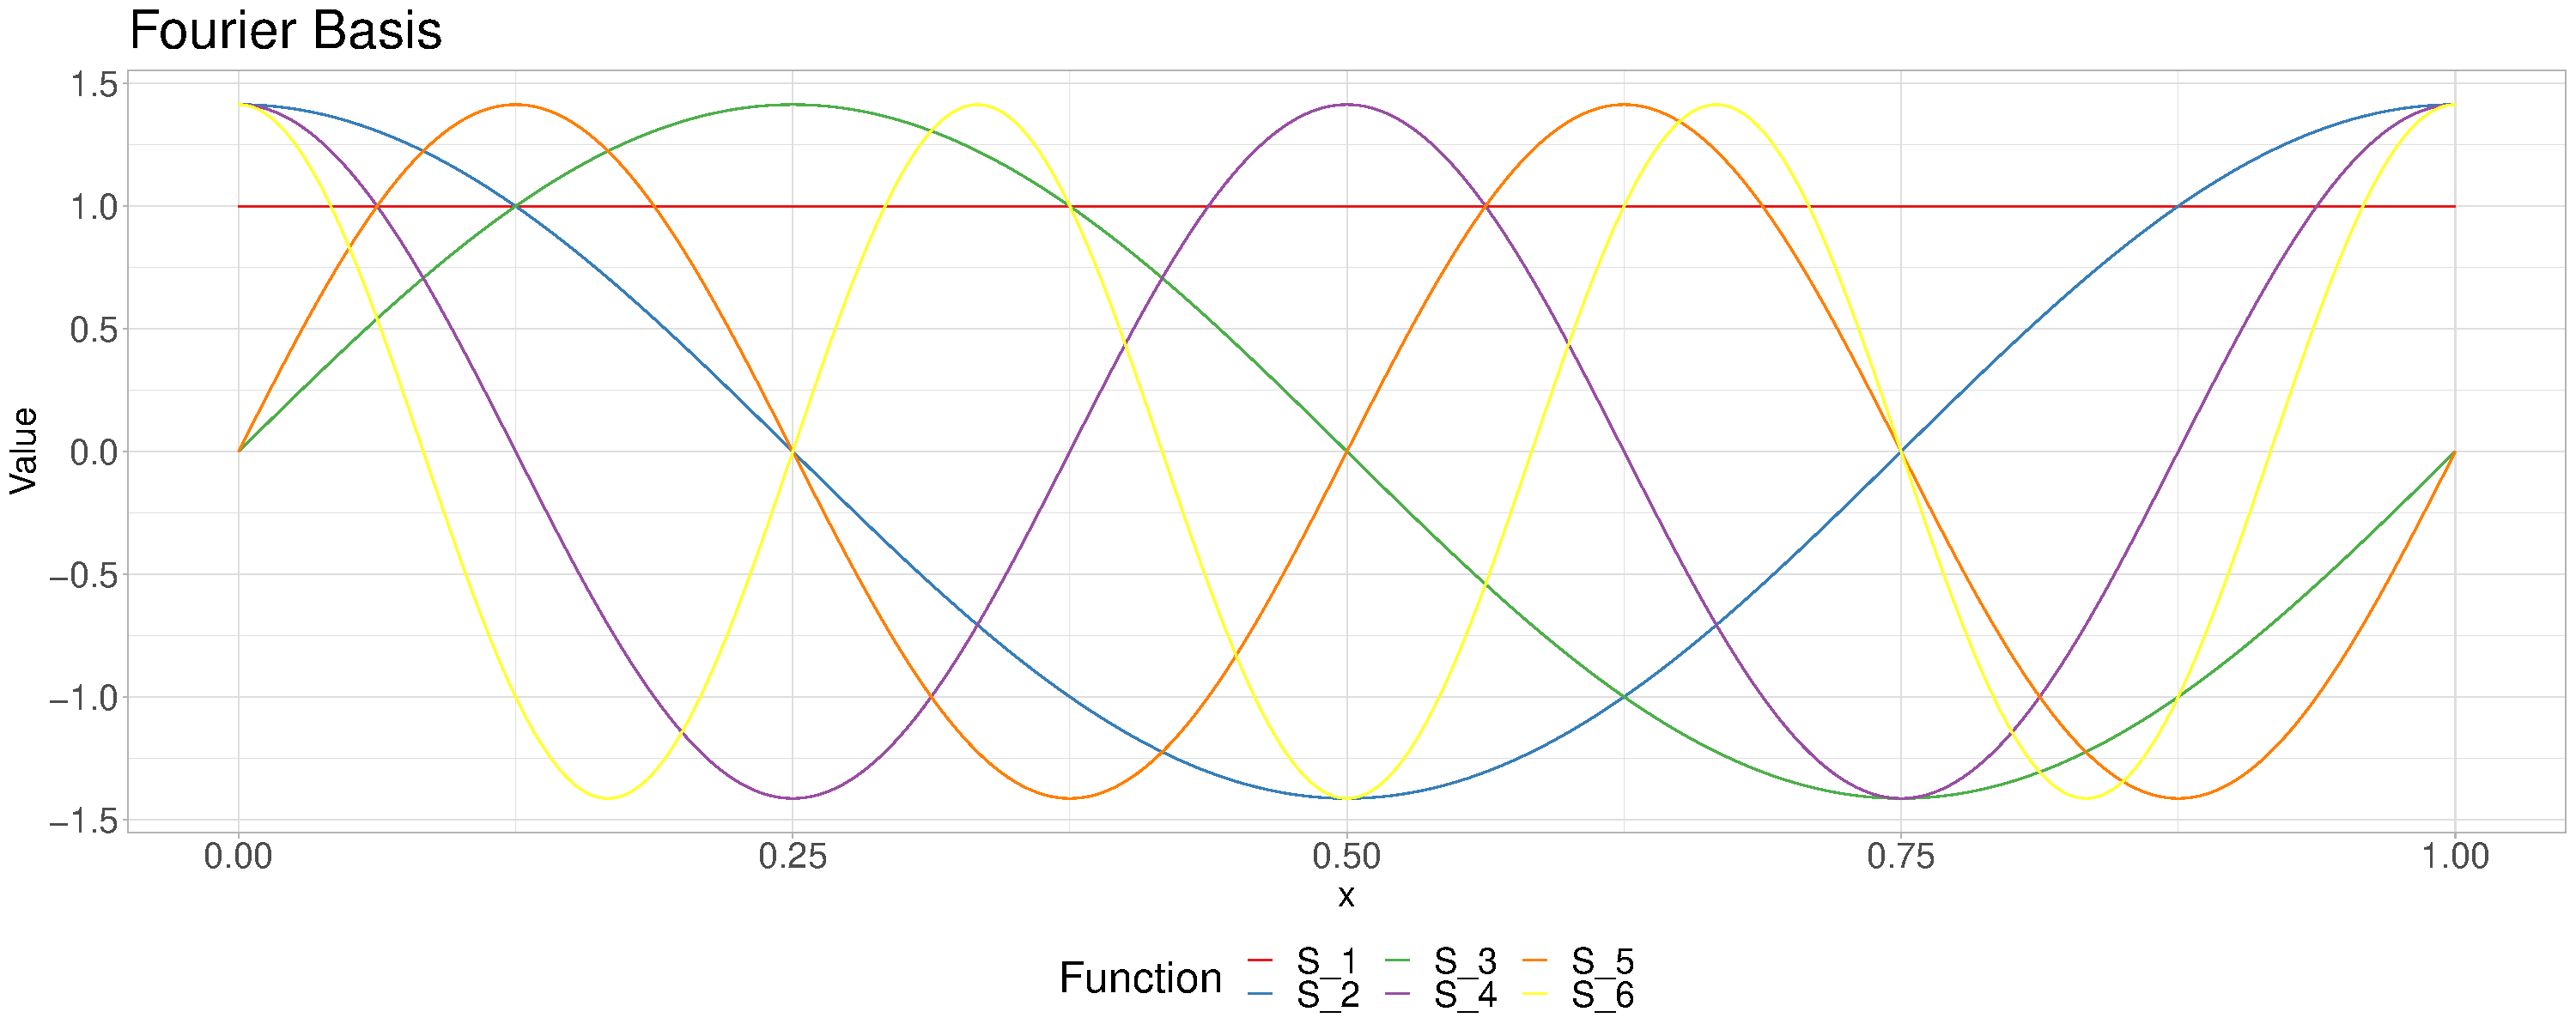
\includegraphics[width = \textwidth]{Graphics/Fourier_Basis.pdf}
	\caption{Fourier basis functions for $i = 1,\dots,6$}
	\end{figure}

	\paragraph{B-spline Basis} Following chapter 3.5 from \cite{ramsay_functional_2005}, splines are defined by first dividing the interval of interest $[\tau_0, \tau_L]$ into $L$ subintervals of non-negative length divided by a non-decreasing sequence of points $(\tau_l)_{l = 1,\dots, L-1}$ called knots. On each subinterval, a spline is a polynomial of chosen order $m = n+1$ where $n$ is its degree. Additionally, at each $\tau_l$ the the polynomials on neighbouring subintervals must match derivatives up to order $m-2$.
	A B-spline is a spline belonging to a basis system developed by \cite{de_boor_practical_1978}. Let $S_{l,m}^{BS}(x) \quad l = 1,\dots,L-1$ be the B-spline of order $m$ for an interval $[\tau_0, \tau_L]$ and knots $\{\tau_l \: \vert \: l = 1,\dots, L-1\}$, then it is defined by the Cox-de Boor recursion formula as follows. 

	\begin{equation}
		\begin{split}
			S_{l,0}^{BS}(x) = &
			\begin{cases}
				1 & \text{if} \quad x \in \left[\tau_l, \tau_{l+1}\right)\\
				0 & \text{otherwise}
			\end{cases}\\ \\
			S_{l,m}^{BS}(x) = &\frac{x - \tau_l}{\tau_{l+m} - \tau_l} S_{l,m-1}^{BS}(x) + \frac{\tau_{l+m+1} - x}{\tau_{l+m+1} - \tau_{l+1}} S_{l+1,m-1}^{BS}(x)
		\end{split}
	\end{equation}
	
	This, however, does not really yield a basis of $\mathbb{L}^2[0,1]$ as the closed span of this finite sequence of functions is not equal to $\mathbb{L}^2[0,1]$. To really obtain a basis of $\mathbb{L}^2[0,1]$ from B-splines, further theoretical considerations about, for example, infinite series of B-splines and specific knot choices would have to be made. As this is out of the scope of this paper, for the sake of simplicity, we will assume that a B-spline basis representation of a function in $\mathbb{L}^2[0,1]$ will serve as a sufficient approximation for an appropriately chosen B-spline basis. 
	Even though, this approach is not theoretically exact, in practice, this is often a reasonable approach and yields satisfactory results in cases where the functional form of B-splines makes them an appropriate approximation tool. 
	
	{\color{red}Explain what happens when $l+m+1 > L$ !!!\\
		Additionally, modify for multiple knots at the boundaries to get better behavior at the boundaries. Needs some more explanation.}

	\begin{figure}[H]\label{bspline_basis}
		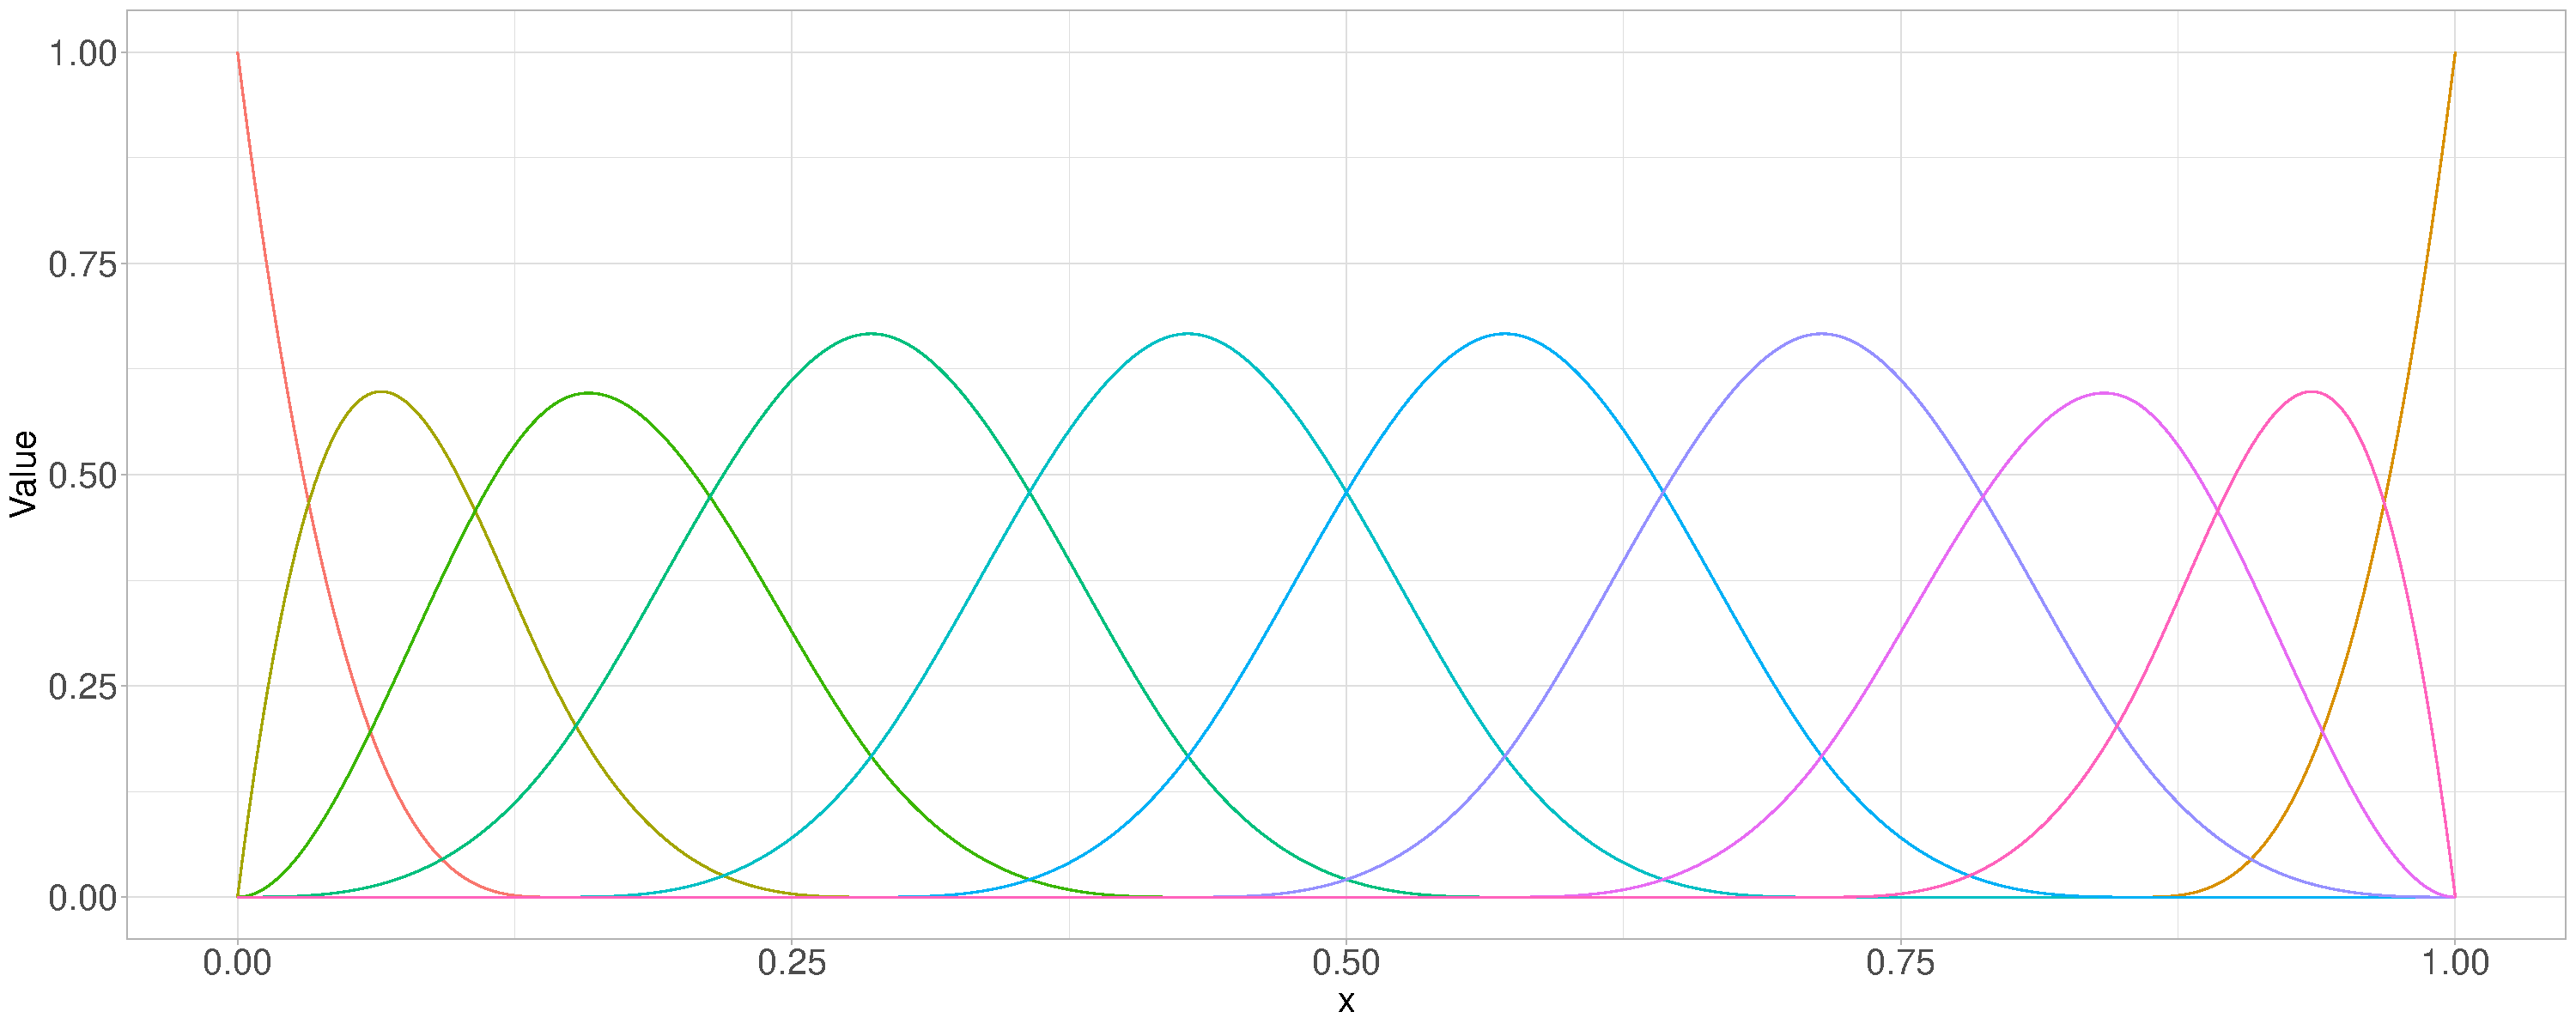
\includegraphics[width = \textwidth]{Graphics/Bspline_Basis.pdf}
		\caption{B-spline basis functions of order 3 for 6 equidistant knots on $[0,1]$}
	\end{figure}
	
	
	\subsection{Approximation and Smoothing via Basis Truncation}
	{\color{red} Write something about how to approximate functions by truncating the basis.}
	
	\begin{equation}
		F(\omega_0) = f(t) = \sum_{j \in \mathcal{I}} \psi_j(\omega_0) b_j(t) = \sum_{j = 1}^{L} \psi_j(\omega_0) b_j(t) + \delta(t) \approx \sum_{j = 1}^{L} \psi_j(\omega_0) b_j(t)
	\end{equation}
	
	\subsection{Functional Data Sets}
	In functional data analysis the concept of a data set can include not only realizations of scalar random variables, but also realizations of random functions. In the following, all random functions are assumed to realize in $\mathbb{L}^2$. As in the finite dimensional setting the concept of identically distributed and independent data is important. This concept generalizes intuitively to the case of functional data using the concepts for general random variables. {\color{red} Explain this better!}\\
	An example of one such data set could be a set of $n$ independent realizations of a Wiener-process and $n$ associated scalar variables that could be subject of a regression analysis with respect to the corresponding realizations of the Wiener process. A definition and a plotted example for the Wiener process are given in \ref{Wiener}.
	
	\subsection{Karhunen-Lo\'{e}ve Expansion and Empirical Eigenbases}
	Given a realization of a random function realizing in $\mathbb{L}^2[0,1]$, it is possible to represent this realization in terms of its generating stochastic process. To motivate it, recall the representation of a random vector derived from the spectral decomposition of its covariance matrix. Let therefore $X(\omega)$ be a random vector realizing in $\mathbb{R}^{p}$ with $\mathbb{E}(X(\omega)) = \mu_x$ and $Cov(X(\omega)) = \Sigma_X$. Then $\Sigma_X$ can be expressed in terms of its Eigenvalues and orthonormal Eigenvectors as $\Sigma_X = \Gamma \Lambda \Gamma'$ using its Eigendecomposition.\\
		
	This decomposition can be used to express the random vector $X(\omega)$ in the following way.
	
	\begin{equation}
		X(\omega) = \mu_x + \Gamma \Lambda^{\frac{1}{2}} D(\omega) = \mu_x + \sum_{i = 1}^{p} \sqrt{\lambda_i} D_i(\omega) \gamma_i
	\end{equation}
	
	where $D(\omega)$ is a random vector with $\mathbb{E}(D(\omega)) = 0_p$ and $Cov(D(\omega)) = \mathbb{I}_p$.\\
	
	To obtain the analogous concept for a random function, it is necessary to define the covariance function of a random function realizing in $\mathbb{L}^2[0,1]$. Therefore, let $F: \Omega \mapsto \mathbb{L}^2[0,1]$ be such a random function.
	Then the mean and covariance functions of $F$ are defined as follows.
	
	\begin{equation}\label{MeanFunction}
		\mu(t) = \mathbb{E}\left[ F(\omega)(t) \right]
	\end{equation}
	
	\begin{equation}\label{CovarianceFunction}
		c(t,s) = \mathbb{E}\big[ \left( F(\omega)(t) - \mu(t) \right) \left( F(\omega)(s) - \mu(s) \right) \big]
	\end{equation}

	Theoretical considerations lead to the result that $F$ can be represented in the following form, called its Karhunen-Lo\'{e}ve expansion.
	
	\begin{equation}\label{KarhunenLoeve}
		F(\omega)(t) = \mu(t) + \sum_{j = 1}^{\infty} \xi_j(\omega) \nu_j(t)
	\end{equation}

	where the $\nu_j$ are defined by the countable set of solutions $\{(\lambda_i, \nu_i) \: \vert \: i \in \mathbb{N}\}$ of the following equation.
	
	\begin{equation}
		\int_{0}^{1}c(t,s)\nu(s) \mathrm{d}s = \lambda \nu(t)
	\end{equation}
	
	The $\xi_j(\omega)$ are then given as $\xi_j(\omega) = \langle F(\omega) - \mu, \nu_j\rangle$ and thereby random variables realizing in $\mathbb{R}$ and have the following properties akin to $\Lambda^{\frac{1}{2}} D(\omega)$ for the case of a random vector.
	
		\begin{multicols}{2}
		\begin{enumerate}
			\item $\mathbb{E}\left[\xi_j(\omega)\right] = 0$
			\item $Var\left(\xi_j(\omega)\right) = \lambda_i$
			\item $Cov\left(\xi_j(\omega), \xi_k(\omega)\right) = 0$ if $j \neq k$
		\end{enumerate}
	\end{multicols}
	
	In the typical scalar setting, a similar consideration leads to the concept of principal components. This is also possible in a functional setting. Let $\{f_1(t), \dots, f_n(t)\}$ be a set of i.i.d. realizations generated by a random function $F(\omega) \mapsto \mathbb{L}^2[0,1]$.
	Define the following sample analogues for the mean and covariance functions.
	
	\begin{equation}
		\hat{\mu}(t) = \frac{1}{n}\sum_{j = 1}^{n}f_j(t)
	\end{equation}

	\begin{equation}
		\hat{c}(t,s) = \frac{1}{n} \sum_{j = 1}^{n} \left(f_j(t) - \hat{\mu}(t)\right) \left(f_j(s) - \hat{\mu}(s)\right)
	\end{equation}

	With these it is possible to derive a set of sample analogs $\{(\hat{\lambda}_i, \hat{\nu}_i) \: \vert \: i \in \mathbb{N}\}$ for $\{(\lambda_i, \nu_i) \: \vert \: i \in \mathbb{N}\}$ as the solutions of the following equation. {\color{red} I think the number of principal components has to be smaller then the number of observations. So I can give more information about $\mathbb{N}$.}
	
	\begin{equation}
		\int_{0}^{1}\hat{c}(t,s)\hat{\nu}(s) \mathrm{d}s = \hat{\lambda} \hat{\nu}(t)
	\end{equation}
	
	This naturally leads to the following representation.
	
	\begin{equation}
		f_i(t) = \sum_{j = 1}^{{\color{red} !!!}} \hat{\xi}_{i,j} \hat{\nu}(t)
	\end{equation}
	
	\subsection{Scalar-on-Function Regression}
	In the simple scalar setting one of the most important tools in econometrics is the linear regression. Its goal is to predict the value of a dependent variable given a set of associated variables. For reference assume a data generating process as follows. {\color{red} Structure is bad... This will be changed.}
	
	\begin{equation}
		Y = X\beta + \epsilon
	\end{equation}
	
	Where $Y$ is the vector of response variables, $X$ is the matrix containing the corresponding regressors in its columns and $\beta = (\beta_0, \beta_1, \: \dots, \beta_p)'$ is the vector containing the unknown coefficients.
	In this finite dimensional setting one important question is how to estimate the unknown coefficients $\beta$. The most well known estimator in all of econometrics, the Ordinary Least Squares (OLS) estimator, fulfills this purpose under a set of assumptions. {\color{red}List Assumptions? Then we need to list the assumptions for functional linear regression as well I think.}
	
	\begin{equation}
		\hat{\beta}_{OLS} = (X'X)^{-1}X'Y
	\end{equation}
	
	The concept of linear regression can be extended to a setting of functional data, where a scalar response variable is supposed to be predicted from a functional variable. 
	A general data generating process in this functional scenario could look like the following equation.
	
	\begin{equation}
		Y(\omega) = \alpha + \Psi\left(F(\omega)\right) + \epsilon(\omega)
	\end{equation}
	
	Here $\Psi$ is a functional that maps a realization of a random function in $\mathbb{L}^2[0,1]$ into $\mathbb{R}$. One simple example to illustrate the principle is the maximum $\Psi(f) = \max_{x \in [0,1]}f(x)$.
	However, the typical setup is often as follows mimicking the structure of the multivariate linear model extended from summation to integration. This structure is crucial for the extension of linear regression to the case of functional regressors. Therefore, in this paper we always implicitly assume that a data generating process has the following structure. {\color{red} maybe a better motivation is the one Jona gave: from very dense observations that run into problems of colinearity when using the original OLS estimator}
	
	\begin{equation}\label{DGP}
		Y(\omega) = \alpha + \int_{0}^{1} \beta(s)F(\omega)(s) \mathrm{d}s + \epsilon(\omega)
	\end{equation}
	
	Where $f(t)$ is the realization of a random function in $\mathbb{L}^2[0,1]$ and $\beta(t)$ is an unknown coefficient function. 
	Similar to the finite dimensional setting, an interesting question is how to estimate the unknown function $\beta(t)$ given a data set containing realizations of a random function and associated scalar response variables. However, a simple extension of the OLS estimator to allow for infinite dimensional objects is not possible. Therefore, other options have to be considered.
	
	\subsection{Estimation via Basis-Representation}
	The most common way to make this problem tractable is via a basis representation of $\beta(t)$. Therefore, let $\{b_i(t) \: \vert \: i \in \mathbb{N}\}$ be a basis of $\mathbb{L}^2[0,1]$ and represent $\beta(t)$ in terms of this basis.
	
	\begin{equation}
		\beta(t) = \sum_{j = 1}^{\infty} \psi_j b_j(t)
	\end{equation}
	
	This enables us to write equation \ref{DGP} with $\beta(t)$ represented in this way to obtain a formulation as a sum of scalar random variables $Z_j(\omega)$.
	
	\begin{equation}
		\begin{split}
			Y(\omega) & = \alpha + \int_{0}^{1}\left[\left(\sum_{j = 1}^{\infty} \psi_j  b_j(s)\right) F(\omega)(s) \right]\mathrm{d}s + \epsilon(\omega) \\
			& = \alpha + \sum_{j = 1}^{\infty} \left[\psi_j \textcolor{red}{\int_{0}^{1} F(\omega)(s) b_j(s)\mathrm{d}s}\right] + \epsilon(\omega) \\
			& = \alpha + \sum_{j = 1}^{\infty} \psi_j \textcolor{red}{\langle F(\omega), b_j \rangle} + \epsilon(\omega) 
			  = \alpha + \sum_{j = 1}^{\infty} \psi_j \textcolor{red}{Z_j(\omega)} + \epsilon(\omega)
		\end{split}
	\end{equation}
	
	This representation translates the original problem of regressing a scalar on a continuously observed function to a problem where a scalar is regressed on a countably infinite sequence of regressors. Using a truncation of the basis at some parameter $L$ can be used to make this problem tractable with typical theory from multivariate regression while staying reasonably accurate.
	
	\begin{equation}
			Y(\omega) \approx \alpha + \sum_{j = 1}^{L} \psi_j Z_j(\omega) + \epsilon(\omega)
	\end{equation}
	
	\subsection{Detailed Draft}
	\begin{itemize}
		\item Motivate random functions from introduction and the general concept of random variables
		\item Formalize random function in this context as random variables realizing in a Hilbert space
		\item Introduce $\mathbb{L}^2[0,1]$ as the Hilbert space of square integrable functions on $[0,1]$
		\item Specialize to Hilbert space being $\mathbb{L}^2[0,1]$ for this context
		\item Define mean and covariance function of a random function realizing in $\mathbb{L}^2[0,1]$
		\item Introduce the concept of a basis of a Hilbert space and specialize to $\mathbb{L}^2[0,1]$
		\item Introduce b-spline and Fourier bases
		\item Introduce eigenfunctions and FPCA on the basis of covariance function (Karhunen-Lo\'{e}ve expansion)
		\item explain similarities to Eigenvalues and Eigenvectors of matrix + PCA (fraction of explained variance etc...)
		\item Introduce functional observations in this context as realizations of a random variable realizing in $\mathbb{L}^2[0,1]$
		\item Explain the concept of iid data in a functional setting		
		\item Define point-wise mean (sample), point-wise standard deviation (sample) and sample covariance function
		\item Explain approximations of functional observations using truncated basis representations
		\item Introduce linear operator $L_1$ and sufficient condition associated with it
		\item Motivate Scalar-on-function regression from multivariate linear regression with a scalar response variable
	\end{itemize}

There are several important aspects of functional regression in this functional setting that separate it from usual multiple regression according to \cite{kokoszka_introduction_2017}: In functional linear regression, the aim is not only to obtain an estimate of the function $\beta(s)$ — this estimate also needs to have a useful interpretation. Without it, there might be prediction, but the increase in understanding of the underlying question will be minimal. One aspect of a useful interpretation is that the estimate $\beta(s)$ should not jump in a seemingly random fashion, because an interpretation of this erratic behavior will often be impossible.

	A common setting in non-functional regression is akin to the following. Assume a model as follows:
	
	\begin{equation}
		Y = X'\beta + \epsilon
	\end{equation}

	where $X \in \mathbb{R}^{n\times J}$ is a matrix containing the regressors, $\beta \in \mathbb{R}^J$ is a coefficient vector and $epsilon$ is a vector containing the error term. For simplicity, assume that the data generating process fulfills the Markov assumptions. Then the famous OLS-estimator is given by:
	
	\begin{equation}
		\hat{\beta}_{OLS} = (X'X)^{-1}X'Y
	\end{equation}

	A naive approach to FLR would be to try to generalize this to the functional setting.
	Assuming a data generating process of the form:
	
	\begin{equation}
    	 Y =  \int \beta(s)X(s) \,\mathrm{d}t \ +\epsilon
    \end{equation}

    it becomes clear that we cannot compute the estimate of $\beta(t)$ as we would do in a classical multivariate setup because of the infinite dimensionality of the underlying objects. Where in the finite dimensional setting the OLS estimator can be derived as a method of moments estimator by solving a system of equations of sample moment restrictions, this leads to a system of infinitely many equations in the functional setting. 
    In practice, functional observations are never truly continuously observed. If we assume that the functional observations are observed at a finite set of points $\{t_1, \dots, t_J\}$ this makes the derivation of an OLS estimator possible as before.
    
    \begin{equation}\label{discrete_time_model}
    	Y_i = \sum_{j = 1}^{n} \beta(t_{j})X_i(t_{j}) + \epsilon_{i},
    \end{equation}

    However, this often still results in a large and difficult to solve system of equations. Even if solved, the result is often a noisy function $\hat{\beta}(s)$ that is not useful for interpretation since it does not use the intuition of smooth functions. Another reason why estimation is not feasible using this approach is colinearity.
    Looking at equation \ref{discrete_time_model} and assuming continuous functions $X_i$ it becomes clear that if $t_{j}$ is close to $t_{j'}$, $X_{i}(t_{j})$ is close to $X_{i}(t_{j'})$. Thereby, there will be vectors $X_{i} = (X_i(t_1), \dots, X_i(t_J))'$ that are highly correlated and thus lead to large variances of $\beta$. (cf. ~\cite{kokoszka_introduction_2017})\\
    A different approach is necessary.
    
    Define therefore
    
    \begin{equation}
  		c_{\mathbf{X}}(t,s) = E[\mathbf{X}(t)\mathbf{X}(s)],\: c_{\mathbf{X}\mathbf{Y}}(t) = E[\mathbf{X}(t)\mathbf{Y}], 
    \end{equation}

   Under the assumption that $X$ is independent from $\epsilon$ we obtain

   \begin{equation}
	   c_{\mathbf{X}\mathbf{Y}}(t) = E[\mathbf{X}(t)\int \beta(t)\mathbf{X}(s) \,\mathrm{d}s \ +\epsilon]
   \end{equation}

   \begin{equation}
 	  c_{\mathbf{X}\mathbf{Y}}(t) = E[\int \beta(s) \: \mathbf{X}(s)\mathbf{X}(t) \, \mathrm{d}s \: | \: X]  + E[\epsilon |\mathbf{X}]
   \end{equation}
  
   \begin{equation}
      c_{\mathbf{X}\mathbf{Y}}(t) = \int c_{\mathbf{X}}(t,s) \beta(s) \,\mathrm{d}s
   \end{equation}
   
   In practice, this results in a large and often difficult to solve system of equations. If solved, a  perfect fit is possible,but results in a noisy and erratic function $\hat{\beta}(s)$ that is not useful for interpretation since it does not utilize the intuition of smooth functions (cf.~\cite{horvath_inference_2012}). Another reason why estimation is not feasible using this approach is colinearity.
   If we approximate the scalar-on-functional regression by assuming a set of discrete observation points for all realizations of the data generating process as
   
  	\begin{equation}
    	Y_i = \sum_{j = 1}^{n} \beta(t_{j})X_i(t_{j}) + \epsilon_{i},
    \end{equation} 

	it becomes clear that if $t_{j}$ is close to $t_{j'}$, $X_{i}(t_{j})$ is close to $X_{i}(t_{j'})$ there will be vectors $X_{i} = (X_i(t_1), \dots, X_i(t_J))'$ that are highly correlated and thus lead to large variances of $\beta$. (cf. ~\cite{kokoszka_introduction_2017}) {\color{red} isn't something missing here? Like "and employ standard multivariate linear regression" // Will be done (Jona)}
  	
	\begin{itemize}
		\item Solution: estimation using truncated basis expansion to approximate data (theoretical description)
	\end{itemize}
		
	The simplest approach to regularize the noisy estimate of $\hat{\beta}(s)$	is to expand it with deterministic basis function. Assume 

	\begin{equation}
     	\beta(t) =  \sum_{k=1}^{K} c_{k}B_{k}(t)
    \end{equation}

    to expand
    
    \begin{equation}
    	\int \beta(s)X(s) \,\mathrm{d}t \ = \sum_{k=1}^{K} c_{k} \int B_{k}(t)X_{i}(t)\,\mathrm{d}t =: \sum_{k=1}^{K} x_{ik} c_{k} 
    \end{equation}

    to the linear model of equation 2 with $\mathbf{c} = [\alpha, c_1, c_2,...,c_K]^T$ (corresponding to $\mathbf{\beta}$) estimated by $\mathbf{\hat{c}} = \mathbf{(X^{T}X)^{-1}X^{T}Y}$. Hence, the estimate $\hat{\beta}$ depends on the basis function $B_{k}$ and its corresponding shape, where $K$ is a subjective choice of the researcher. This subjective choice highly depends on the researchers intuition of the smoothness of the estimate. It is best practice to use the same basis functions as in {\color{red} add link to smoothing} (cf. ~\cite{kokoszka_introduction_2017})
    
    {\color{red} include Part about CI´s? its about inference and not about prediction}
    
	\begin{itemize}
		\item Problem: truncation error $\delta$ and how to deal with it?
	\end{itemize}

	\begin{itemize}	
		\item Explain how to address truncation error in standard errors
		\item Motivate three estimation procedures
		\begin{enumerate}
			\item truncated b-spline basis expansion without addressing truncation error
			\item truncated b-spline basis expansion WITH addressing truncation error
			\item truncated Eigenbasis expansion (advantages: low number of basis functions get low approximation error)
		\end{enumerate}
	\end{itemize}
	
	\subsection{Draft-Overview}
	\begin{itemize}
		\item Motivate Karhunen-Loeve-Expansion and Eigenbasis from PCA		
		\item Explain Scalar-on-Function Regression
		\item Estimation through basis-expansion (incl. Eigenbasis) [and estimation with roughness penalty]
		\item Address approximation error due to basis-truncation
	\end{itemize}

	\subsection{Literature}
	\begin{itemize}
		\item \cite{kokoszka_introduction_2017}
		\item \cite{hsing_theoretical_2015}
		\item \cite{ramsay_functional_2005}
		\item \cite{horvath_inference_2012}
		\item \cite{cai_prediction_2006}
		\item \cite{levitin_introduction_2007}
	\end{itemize}
	
	\newpage
	\section{Simulation Study}
	
	\subsection{Draft-Overview}
	\begin{itemize}
		\item Motivate Simulation for some data generating process from application
		\item Describe Simulation Setting from technical standpoint (DGP, set-up for replication, ...)
		
		\item Compare estimation with \begin{enumerate}
			\item b-spline basis without addressing approximation error
			\item ... including proper treatment of approximation error
			\item Eigenbasis constructed from observations
			\end{enumerate}
	
		\item Prediction not Inference (Alternative: Focused on a testing procedure motivated by the application)
		\item Present Results
		\item Explain relevance for application
	\end{itemize}

	\subsection{Motivate Simulation for some data generating process from application}
	For the simulation study, we use the gasoline dataset to predict the octane ratings of gasoline samples relying on the introduced methods. This has become more relevant as modern internal combustion engines become more complex and rely on precisely tuned fuels. The dataset, which contains 60 i.i.d. observations with each 400 measurements, was constructed using Near infra-red (NIR) spectroscopy, which allows to analyse samples of gasoline much faster and with the same reproducibility as standard tests (cf. \cite{Bohacs_Ovadi_Salgo1998}). The study follows Reiss and Ogden (2007) as a guideline. Similar to Reiss and Ogden (2007), two different true coefficient functions $f_1$ and $f_2$ were chosen that differ in their smoothness: 
	
	\begin{equation}
    	f_1 = 2\sin(0.5\pi t) + 4\sin(1.5 \pi t) + 5\sin(2.5 \pi t) 
    \end{equation}

    \begin{equation}
    	f_2 = 1.5^{\frac{-0.5(t-0.3)^2}{0.02^2}} - 4^{\frac{-0.5(t-0.45)^2}{0.015^2}} +  8^{\frac{-0.5(t-0.6)^2}{0.02^2}} -  1^{\frac{-0.5(t-0.8)^2}{0.03^2}}
    \end{equation}

Two different error-terms $\epsilon $ were created by first generating iid standard normal error and then multiplying them by $\sigma_e $ which is calculated such that the squared multiple correlation coefficient $R^2 = var(Xf) / (var(Xf) + \sigma^2_{e})$ is equal to 0.9 and 0.6. The two error-terms are then computed to generate two sets of responses with different signal-to-noise ratios for each true function, using the gasoline dataset. These four combinations are then used with different number of basis-function $(5,6,...,25)$ of the order 5 to predict the responses using the b-spline basis approach and the FPCR approach. Within one repetition, the data is randomly sampled into a training and a test set to calculate the reported test MSE. The simulation was done with R (version...). In total we carried out 2000 simulations for each combination of data and number of basis functions. {\color{green} Information about version and link to repo / package in footnote??}


	\subsection{Generating Similar Curves}
    {\color{blue} I shifted this from theory to over here, as it makes more sense in the simulation part.\\
    Very short summary: take fpc's and eigenvalues, use that the scores are independent from each other. Use the eigenvalues as variances and draw from a multivariate normal with the right varcov matrix (normal just because of convenience... No theoretical reasoning)}
	\subsection{Results}

		\subsubsection{Interpretation and Relevance for Application}

	\subsection{Literature}
	\begin{itemize}
		\item \cite{shonkwiler_explorations_2009}
		\item R-packages: fda, refund, mgcv
	\end{itemize}
	
	\newpage
	\section{Application}
The application uses the insights from the previous sections to predict the octane ratings of the introduced gasoline dataset. Following the results from the simulation study,... 
\begin{itemize}
\item
{\color{green} incorporate results of simulation study: number of basis, components, etc...}
\item
point out difficulties estimating sderror
\item
describe setup and results
\end{itemize}


	\subsection{Draft-Overview}
	\begin{itemize}
		\item Prediction not Inference (Alternative: Focused on a testing procedure motivated by the data set)
		\item IID data set (no dependence between the curves, don't want to do functional time series)
		\item Not necessarily data from economics (like biology, sports, whatever)
		\item Smooth curves or random walk (both fine)
		\item \href{https://functionaldata.wordpress.ncsu.edu/resources/}{https://functionaldata.wordpress.ncsu.edu/resources/}
	\end{itemize}
	
	\subsection{Literature}
	\begin{itemize}
		\item \cite{carey_life_2002}
	\end{itemize}

	\section{Outlook}
	
	\subsection{Literature}
	\begin{itemize}
		\item \cite{James.2009} (shape-restrictions)
	\end{itemize}
	
	\section{Appendix}
	
	\subsection{Wiener Process}\label{Wiener}
	A Wiener process $W_t$ is a real-valued continuous-time stochastic process {\color{red} ... This is wikipedia, look for right citation!}
	It is characterized by the following properties.
	
	\begin{multicols}{2}
		\begin{enumerate}
			\item $W_0 = 0$
			\item $\forall t > 0 W_{t+u} - W_t \perp\!\!\!\perp W_s \forall s \leq t$
			\item $W_{t+u} - W_t \sim \mathcal{N}(0,u)$
			\item $W_t$ is continuous in $t$
		\end{enumerate}
	\end{multicols}

	\begin{figure}[H]\label{Wiener_plot}
		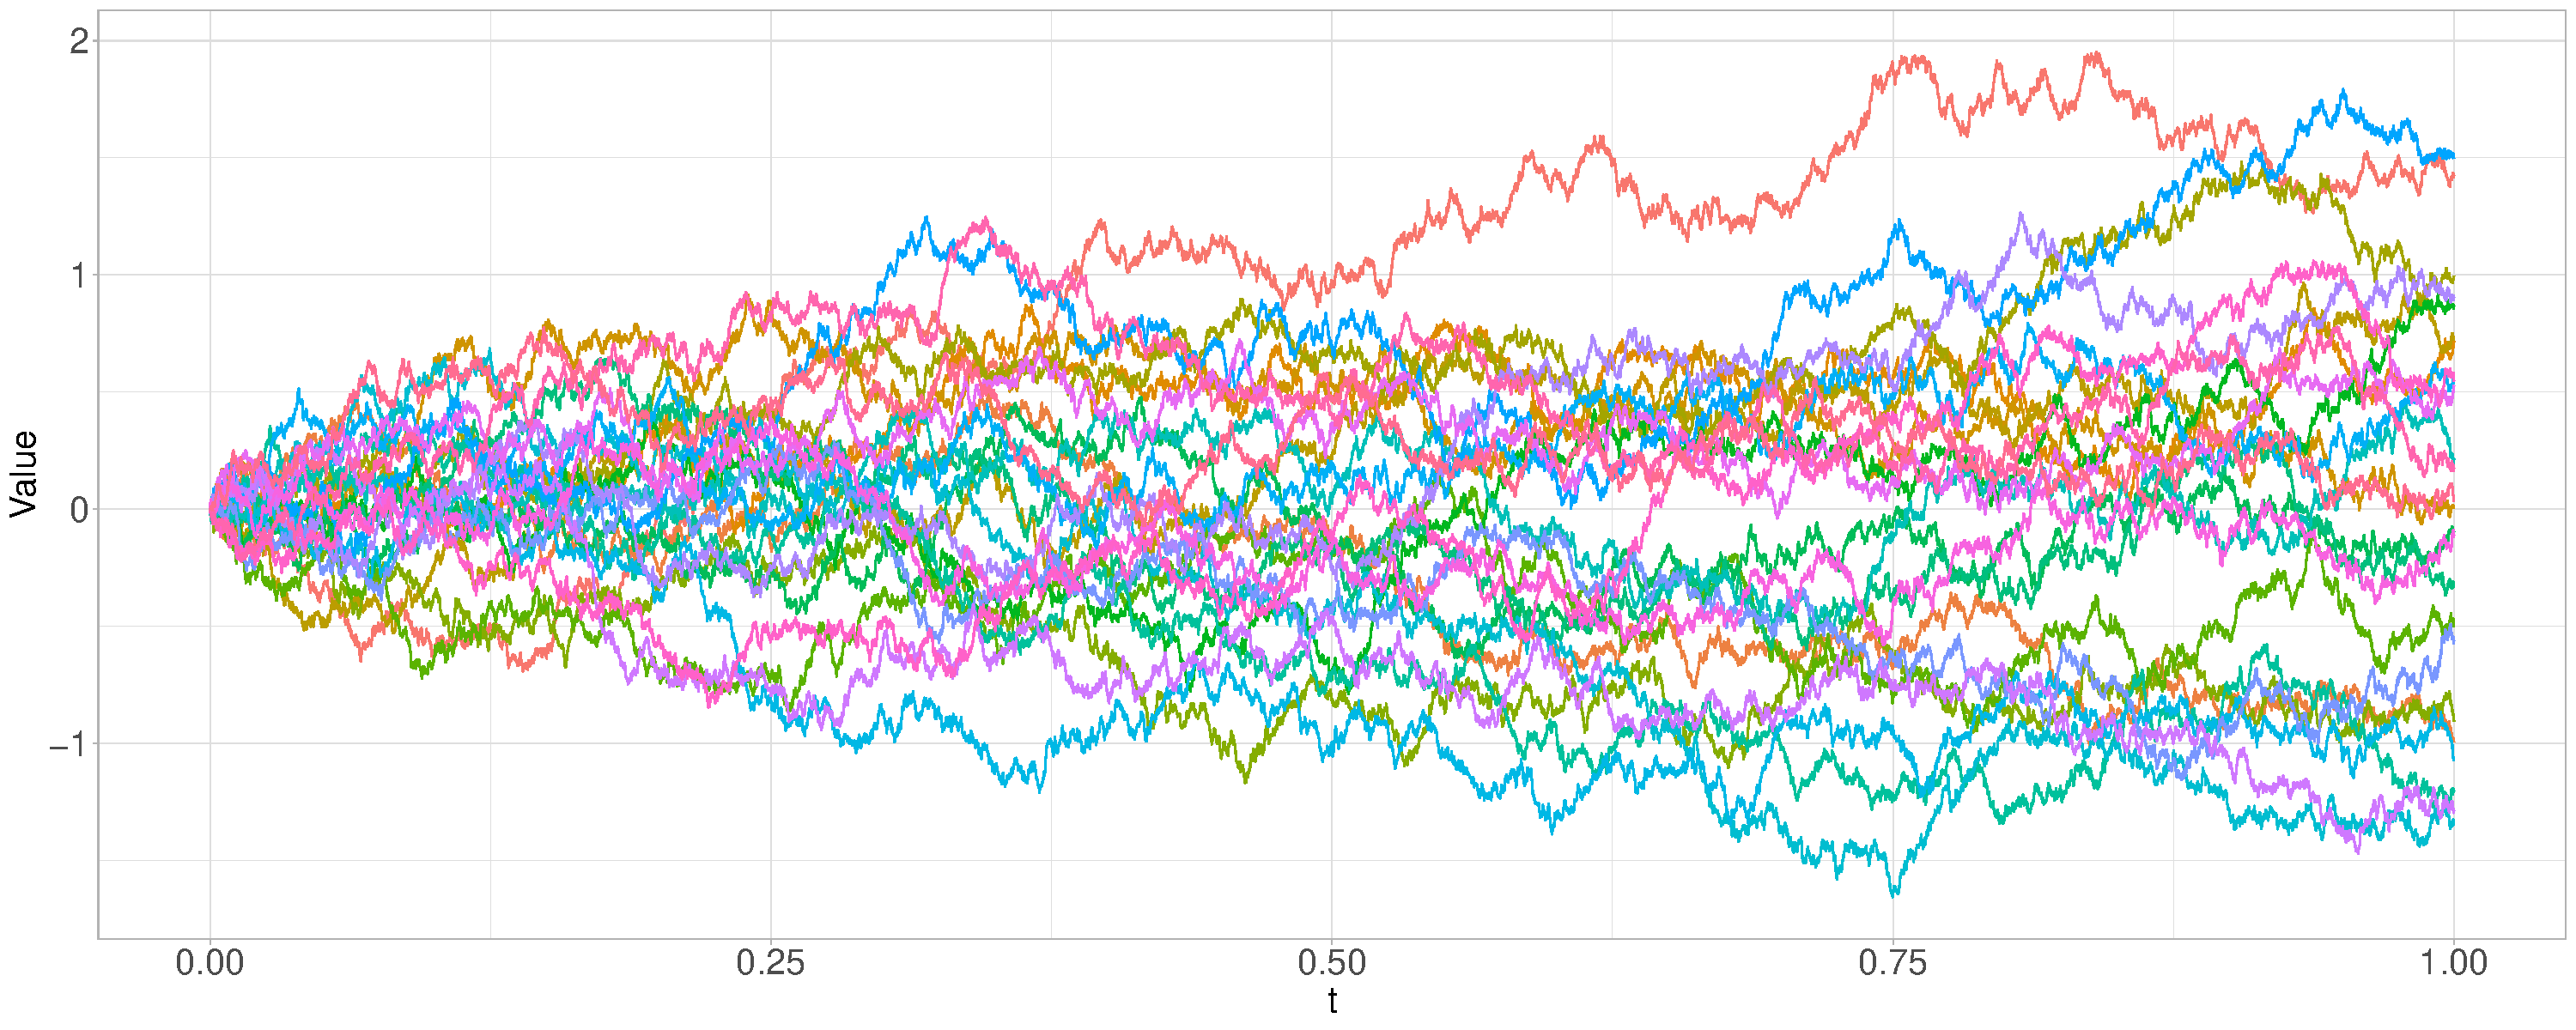
\includegraphics[width = \textwidth]{Graphics/Wiener_plot.pdf}
		\caption{25 i.i.d. realizations of a Wiener Process on $[0,1]$}
	\end{figure}

	\newpage
	
	\section{Bibliography}
	\printbibliography[heading=none]	
	
\end{document}